
\nonstopmode
\documentclass{beamer}

\usepackage{amsmath,amssymb}
\usepackage{algorithm2e}
\usepackage{algorithmic}

% Some useful declarations for equations
\DeclareMathOperator*{\E}{\mathbb{E}}
\newcommand{\prob}{\text{I\kern-0.15em P}}
\newcommand{\argmin}{\arg\!\min}


\setbeamertemplate{navigation symbols}{}

\usepackage{beamerthemeshadow}
\begin{document}
\title{Markov Chains}  
\author{Dr. João Victor da Fonseca Pinto}
\date{\today} 

\begin{frame}
\titlepage
\end{frame}

\begin{frame}
    \frametitle{Table of contents}
    \tableofcontents
\end{frame} 



\begin{frame}
    \frametitle{Introduction}

    In real life, we work with data that are affected by randomness, and 
    we need to extract information and draw conclusions from the data.
    \begin{itemize}

        \item Suppose that we would like to predict the outcome of an election. 
        Since we cannot poll the entire population, we will choose a random sample 
        from the population and ask them who they plan to vote for. 
        In this experiment, the randomness comes from the sampling. 
        
        \item Note also that 
        if our poll is conducted one month before the election, another source of 
        randomness is that people might change their opinions during the one month 
        period.
    \end{itemize}
\end{frame}



\begin{frame}
    \frametitle{Introduction}

    \begin{itemize}
        \item \textbf{Frequentist (classical) Inference:} Based on the samples (random variable $X$)
        we can propose some distribution with unknown (fixed) parameter $\theta$ that best describe the population.

        \item \textbf{Bayesian Inference:} Inthe bayesian approch, $\theta$ is a random variable.

    \end{itemize}
\end{frame}



\begin{frame}
    \frametitle{Introduction: Basic Statistical Concepts}
    \begin{definition}
        A random variable $X$ is a function from the sample space to the real numbers.
        $$X: S\rightarrow\mathbb{R}$$
    \end{definition}
\end{frame}

\begin{frame}
    Toss a coin five times. This is a random experiment and the sample space can be written as

    $$S = \left{TTTTT, TTTTTH, ..., HHHHHH\right}$$

    in this experiment, we are interested in the number of heads. We can define a random variable $X$
    whose value is the number of observed heads. 

    $$X = [0,1,2,3,4,5]$$

    depending on the outcome of the random experiment.

\end{frame}


\begin{frame}
    \frametitle{Introduction: Basic Statistical Concepts}
    \begin{figure}
        \centering
        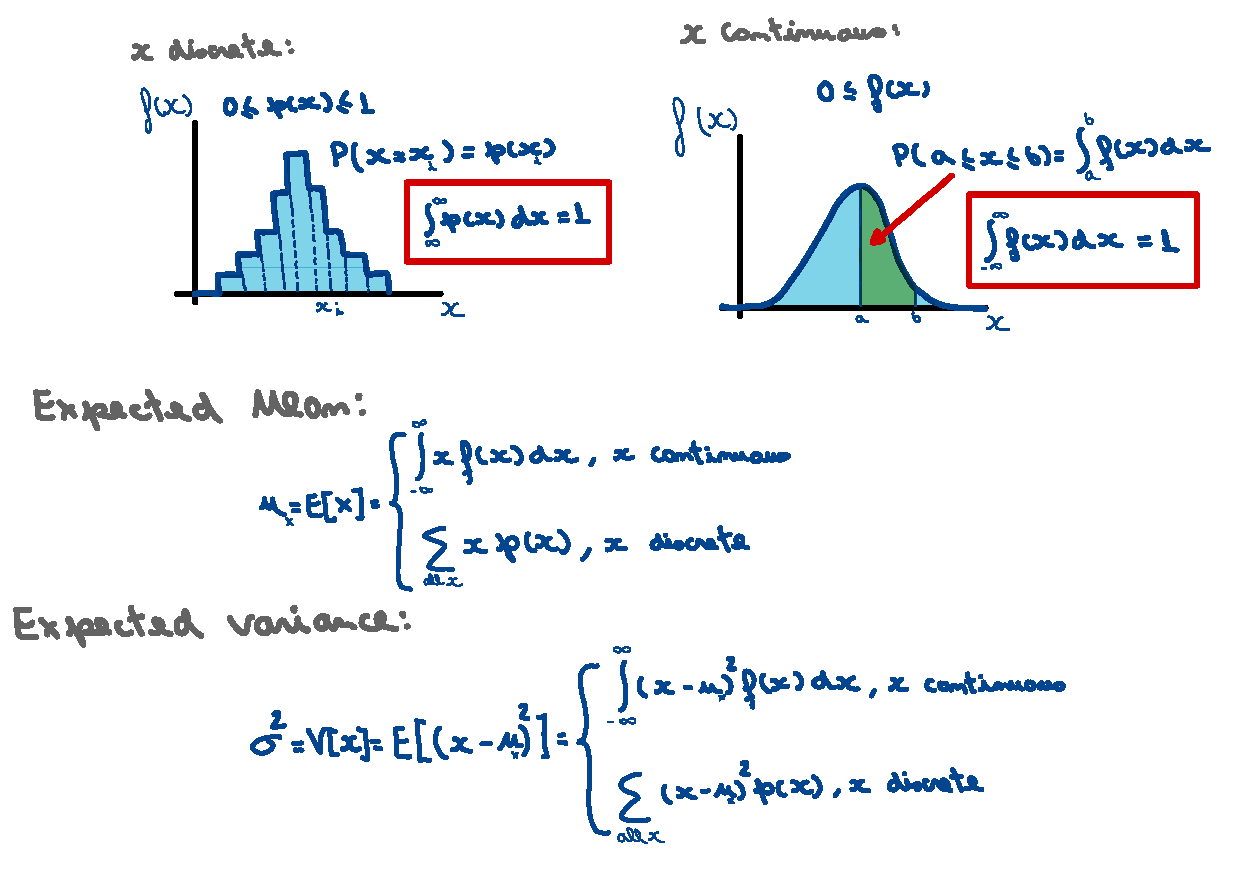
\includegraphics[width=1\textwidth]{slides/figures/prob_review_part_one.pdf}
    \end{figure}
\end{frame}

\begin{frame}
    \frametitle{Introduction: Basic Statistical Concepts}
    \begin{figure}
        \centering
        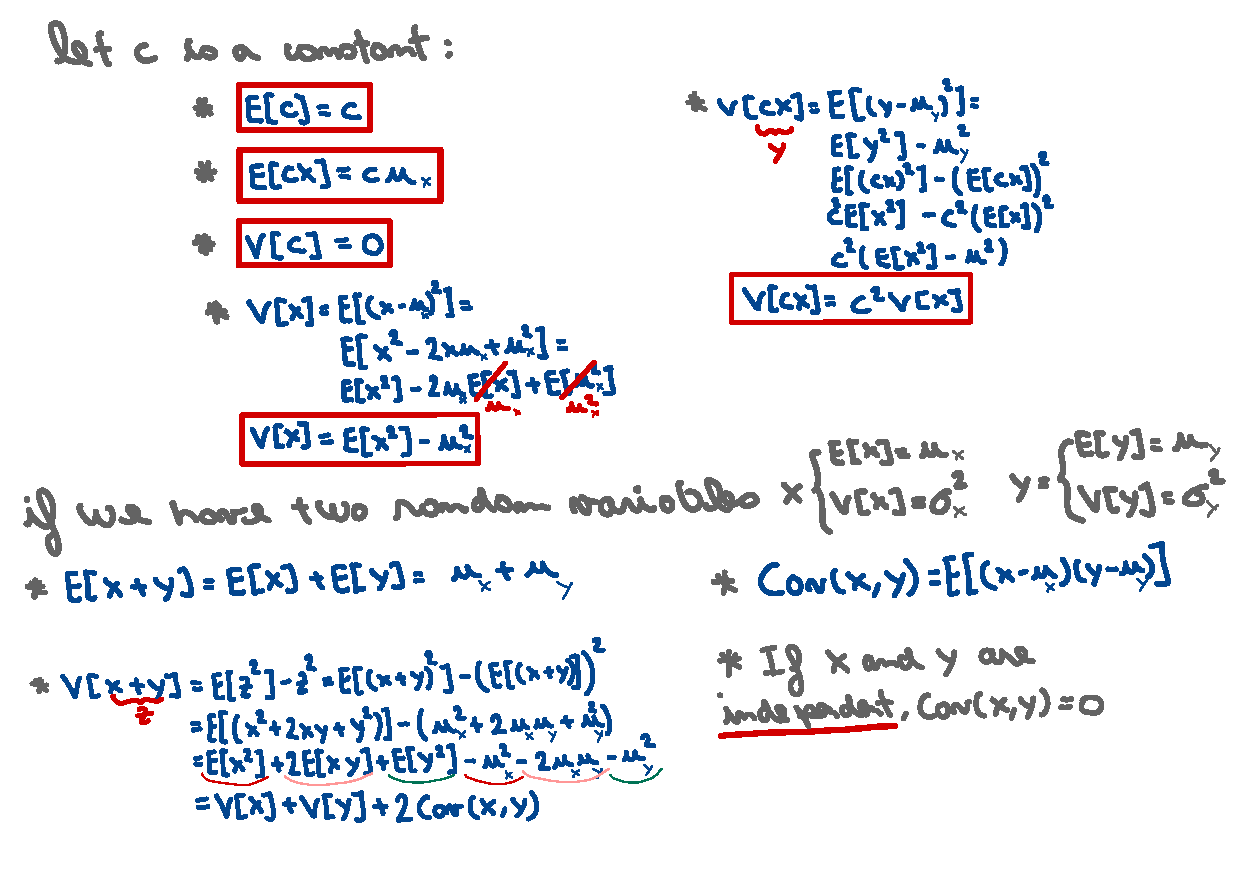
\includegraphics[width=1\textwidth]{slides/figures/prob_review_part_two.pdf}
    \end{figure}
\end{frame}


\begin{frame}
    \frametitle{Sampling from Pratical Example}

    Our goal is to investigate the height distribution of people in a well defined population 
    We choose a random sample of size $n$ \textbf{with replacement from the population} and let $X_i$
    be the height of the $i$th chosen person. More specifically,
    \begin{itemize}
        \item We chose a person uniformly at random from the population and let $X_1$
        be the height of that person. Here, every person in the population has the same chance of being chosen.

        \item o determine the value of $X_2$, again we choose a person \textbf{uniformly} 
        (and \textbf{independently from the first person}) at random and let $X_2$
        be the height of that person. Again, every person in the population has the same chance of being chosen.

        \item In general, $X_i$ is the height of the $i$th person that is \textbf{chosen uniformly and independently} 
        from the population.

    \end{itemize}
\end{frame}



\begin{frame}
    \frametitle{Sampling}

    \begin{itemize}
        \item You might ask why do we do the sampling with replacement?

        \item In practice, we often do the sampling without replacement, that is, we do not allow one person 
        to be chosen twice. If the population is large, then the probability of choosing one person twice is extremely low.

        \item The big advantage of sampling with replacement is that $X_i$'s will be independent and this makes 
        the analysis much simpler.

    \end{itemize}
\end{frame}

\begin{frame}
    \frametitle{Sampling}

    \begin{definition}
        The collection of random variables $X_1, X_2, ..., X_n$
        is said to be a \textbf{random sample} of size $n$ if they are independent and identically distributed (i.i.d.), i.e.,

        \begin{itemize}
            \item $X_1, X_2, ..., X_n$ are independent \textbf{random variables}, and
            \item they have the same distribution, i.e,
            $$f_{X_1}(x) = f_{X_2}(x) = ... = f_{X_n}(x)~~\text{for all $x\in\mathbb{R}$}$$
        \end{itemize}

    \end{definition}
\end{frame}



\begin{frame}
    \frametitle{Sampling: Sample Mean and Sample Variance}

    Statistical inference makes considerable use of quantities computed from the observations in the sample.
    \begin{itemize}
        \item \textbf{Sample mean:} The mean \textbf{estimator} is defined as

        $$\overline{x} = \frac{1}{n}\sum_{i=1}^{n}x_i$$

        \item \textbf{Sample variance:} The variance \textbf{estimator} is defined as
        $$S^2 = \frac{1}{n-1}\sum_{i=1}^{n}(x - \overline{x})^2$$

        Sometimes $S=\sqrt{S^2}$, called the \textbf{sample standard deviation}, is used
        as a measure of dispersion.
    \end{itemize}
\end{frame}




\begin{frame}
    \frametitle{Point Estimation}

    A point estimator is a random variable.
    \begin{itemize}
        \item The \textbf{sample} mean ($\overline{x}$) is a \textbf{point estimation} of the
        \textbf{population} mean ($\mu$). 

        \item The \textbf{sample} variance ($S^2$) is a \textbf{point estimation} of the
        \textbf{population} variance ($\sigma^2$).
    \end{itemize}

    Several properties are required of \textbf{good point estimators}. 
    Two of the most important are the following:

    \begin{itemize}
        \item \textbf{Unbiased:} The expected value of the point estimator should be equal to the 
        parameter that is being estimated.
        \item \textbf{Minimum variance:} The variance point estimator has a variance that is smaller 
        than the variance of any other estimator of that parameter.
    \end{itemize}

\end{frame}

\begin{frame}

    We may easily show that $\overline{x}$ and $S^2$ are unbiased estimators of $\mu$ and $\sigma^2$, respectively.
    \begin{figure}
        \centering
        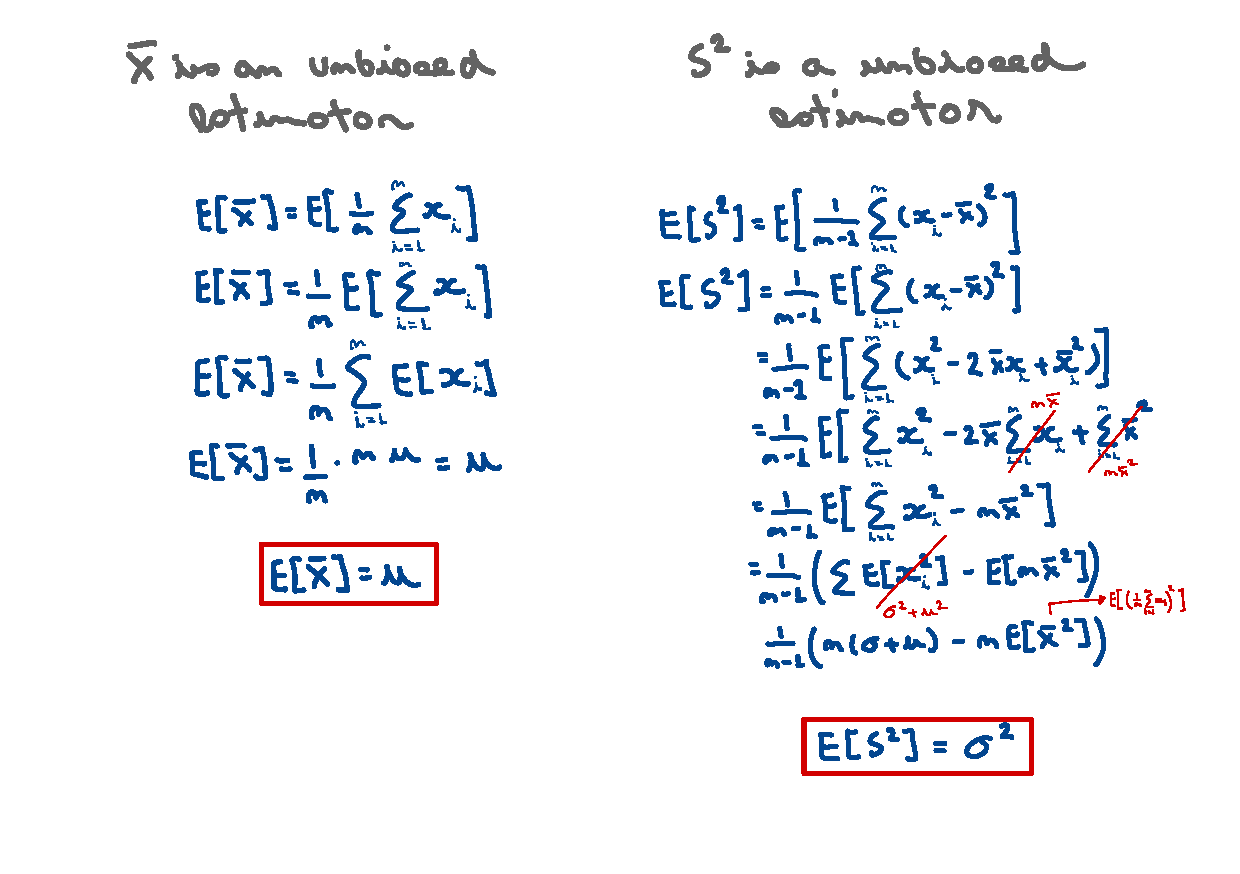
\includegraphics[width=1\textwidth]{slides/figures/mean_and_variance_unbiased_proof.pdf}
    \end{figure}

    The quantity $n-1$ (variance sample) or $n$ (mean sample) is called the number of \textbf{degrees of freedom}.

\end{frame}






\begin{frame}
    \frametitle{The Normal Distribution}

    %we are able to determine the probability distribution of a particular 
    %statistic if we know the probability distribution of the population from which the sample was drawn.
    \begin{itemize}
    
        \item The probability distribution of a statistic is called a \textbf{sampling distribution}.

        \item the most important sampling distributions is the normal distribution. 
        If $x$ is a normal random variable, the probability distribution of $x$ is

        $$f(x) = \frac{1}{\sigma\sqrt{2\pi}}e^{-0.5\left(\frac{x-\mu}{\sigma}\right)^2}~~\text{, $\infty < x < \infty$}~{\color{red}\Rightarrow~N(\mu,\sigma^2)}$$

        \item We can also map any random variable $x$ described by the normal distribution to the standard normal
        distribution, using
        $$z = \frac{x-\mu}{\sigma}~\text{where we map} ~{~\color{red}N(\mu,\sigma^2)\rightarrow~N(0,1)}$$

    \end{itemize}
\end{frame}

\begin{frame}
    \frametitle{The Central Limit Theorem (CLT)}
    \begin{definition}
        If $X_1,X_2,...,X_N$ is a sequence of $n$ independent and identically distributed 
        random variables with $E[X_i]=\mu$ and $V[X_i]=\sigma^2$ (both finite) and $Y=X_1+X_2+...+X_n$, then 
        the limiting form of the distribution of

        $$Z_n = \frac{Y-n\mu}{\sigma\sqrt{n}}$$

        as $n\rightarrow\infty$, is the \textbf{standard normal distribution}.

    \end{definition}
\end{frame}



\begin{frame}
    \frametitle{The Central Limit Theorem (CLT)}

    \begin{figure}
        \centering
        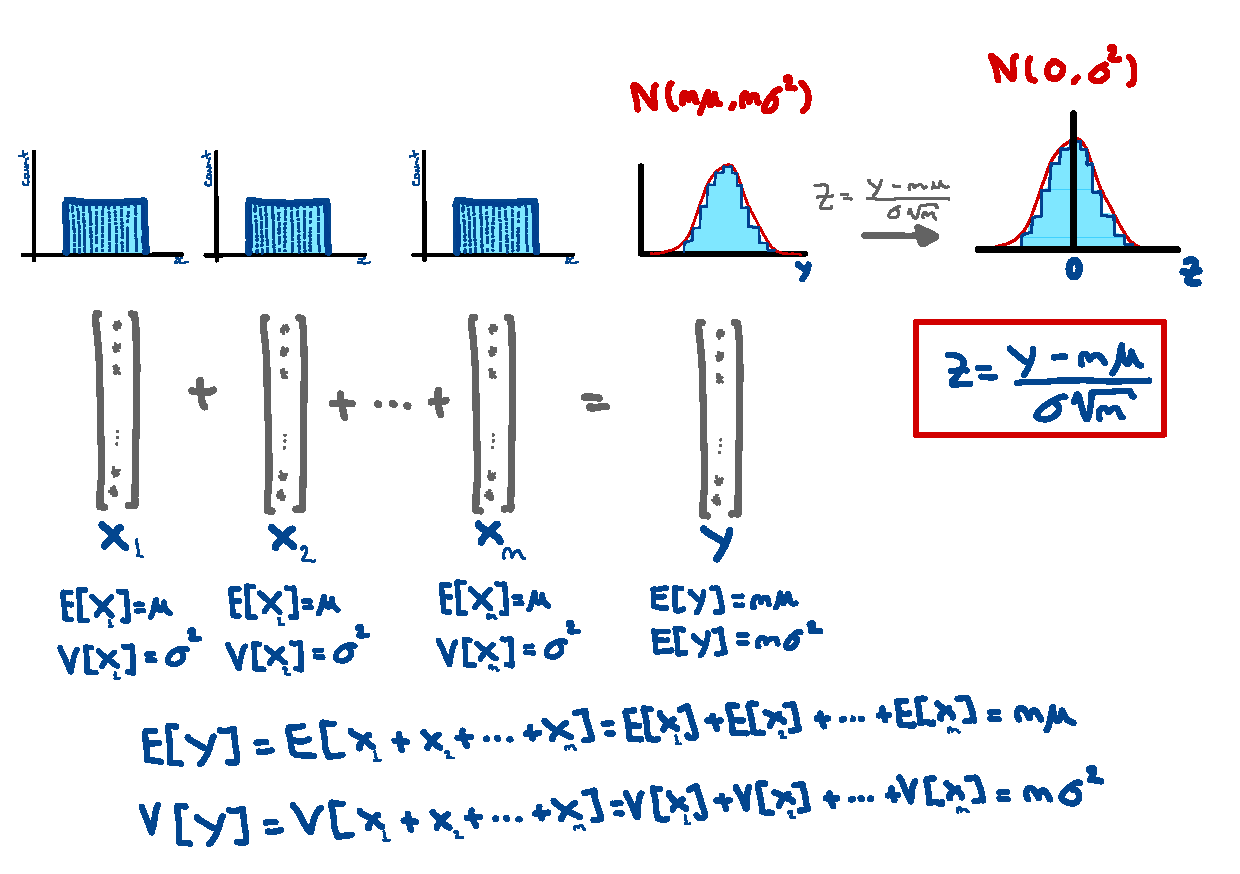
\includegraphics[width=1\textwidth]{slides/figures/clt_examples.pdf}
    \end{figure}

\end{frame}



\begin{frame}
    \frametitle{Confidence Intervals}
    \begin{definition}[Interval estimation]
        Let $X_1$, $X_2$, ..., $X_n$ be a random sample from a distribution with parameters $\theta$ that 
        is to be estimated. As \textbf{interval estimator} with \textbf{confidence level} $1-\alpha$
        consists of two estimators $\hat{\theta}_h(X)$ and $\hat{\theta_h}(X)$ such that

        $$P(\hat{\theta}_l \leq \theta \leq \hat{\theta}_h ) \geq 1-\alpha$$

        for every possible value of $\theta$.

    \end{definition}


\end{frame}



\begin{frame}
    \frametitle{Confidence Intervals for large samples: Example}
    Let $Z\rightarrow N(0,1)$, find $x_l$ and $x_h$ such that $P(x_l \leq Z \leq x_h) = 0.95$
    \begin{figure}
        \centering
        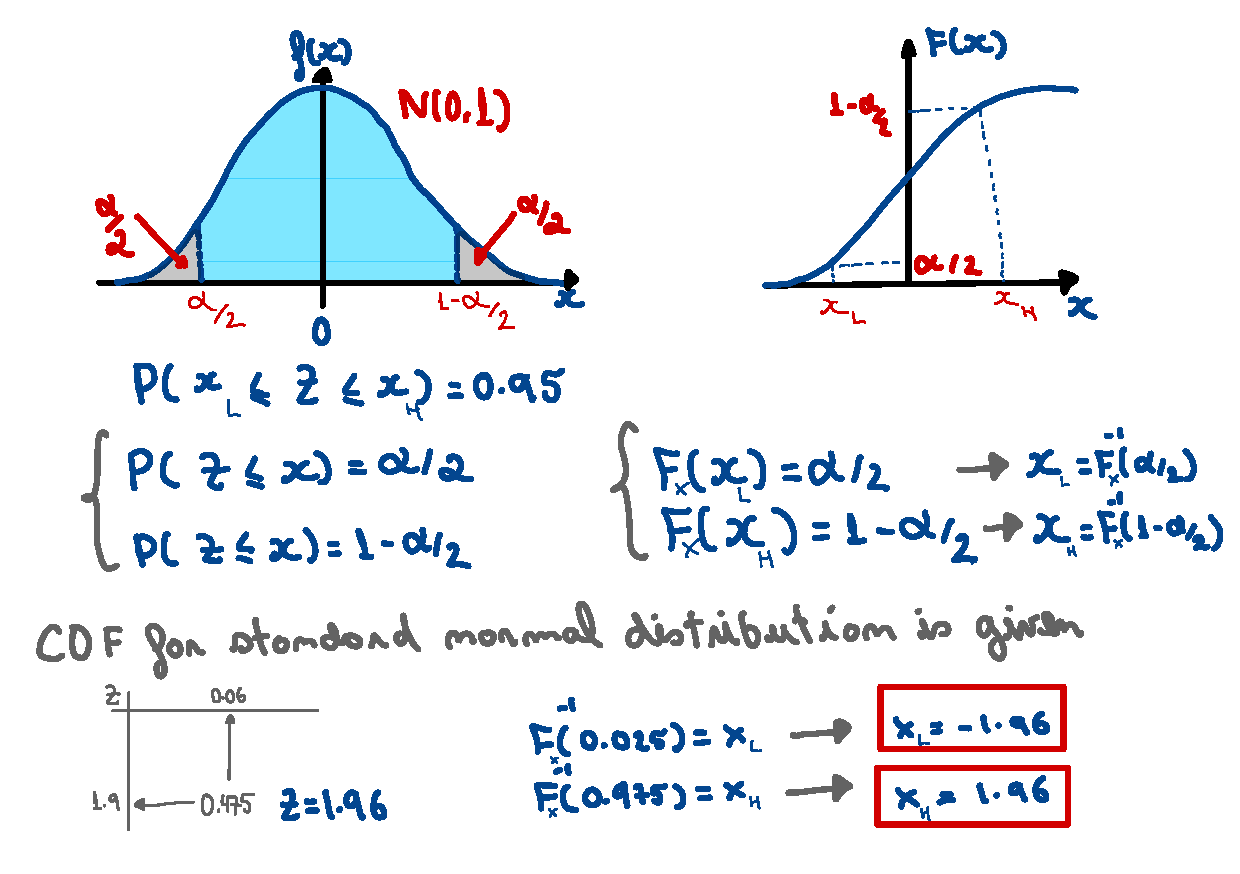
\includegraphics[width=1\textwidth]{slides/figures/interval_example_one.pdf}
    \end{figure}
\end{frame}

\begin{frame}
    \frametitle{Confidence Intervals: Example}
    Let $x_1, x_2,..., x_i$ be a random sample from a normal distribution ($N(\theta,1)$). Find $95\%$ confidence interval
    for $\theta$
    \begin{figure}
        \centering
        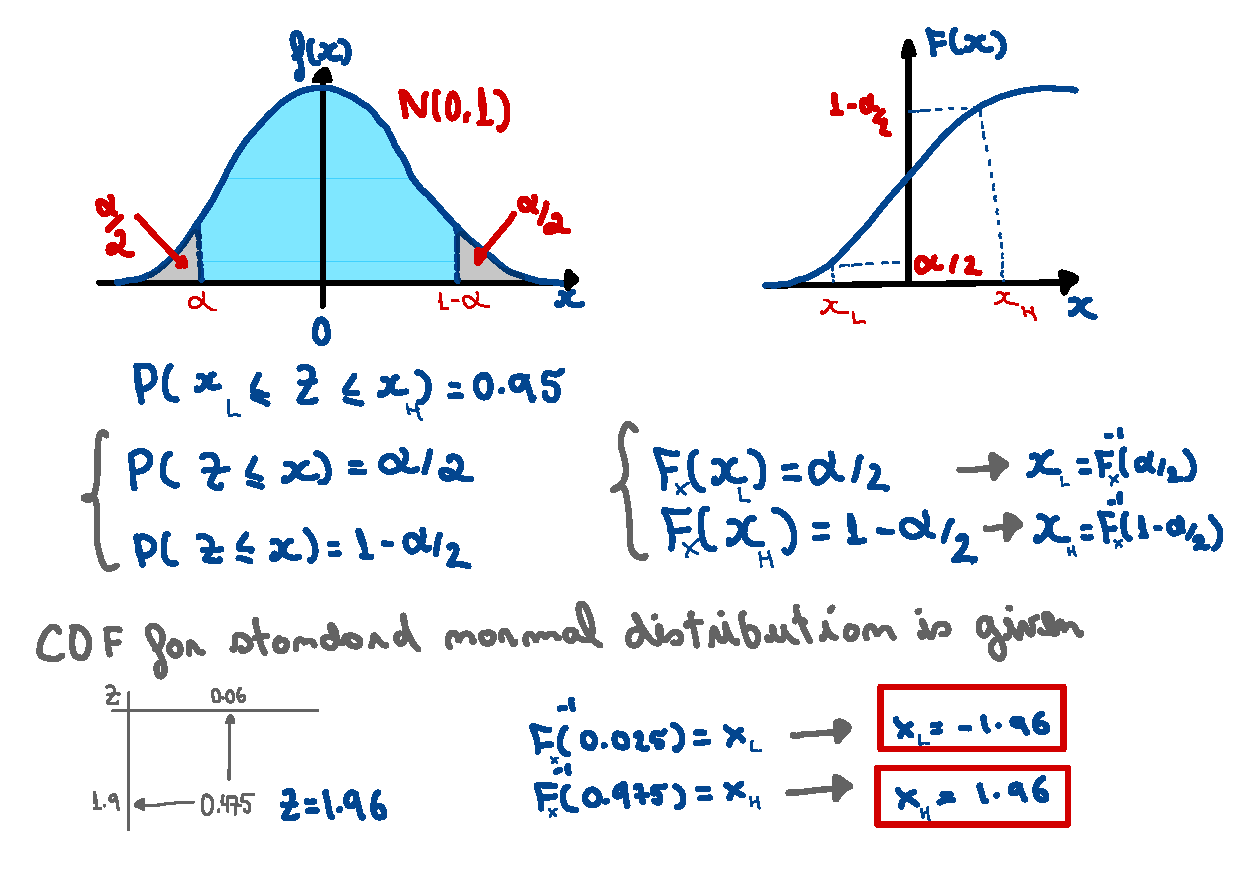
\includegraphics[width=1\textwidth]{slides/figures/interval_example.pdf}
    \end{figure}
\end{frame}


\begin{frame}
    \frametitle{Confidence Intervals}
    \begin{figure}
        \centering
        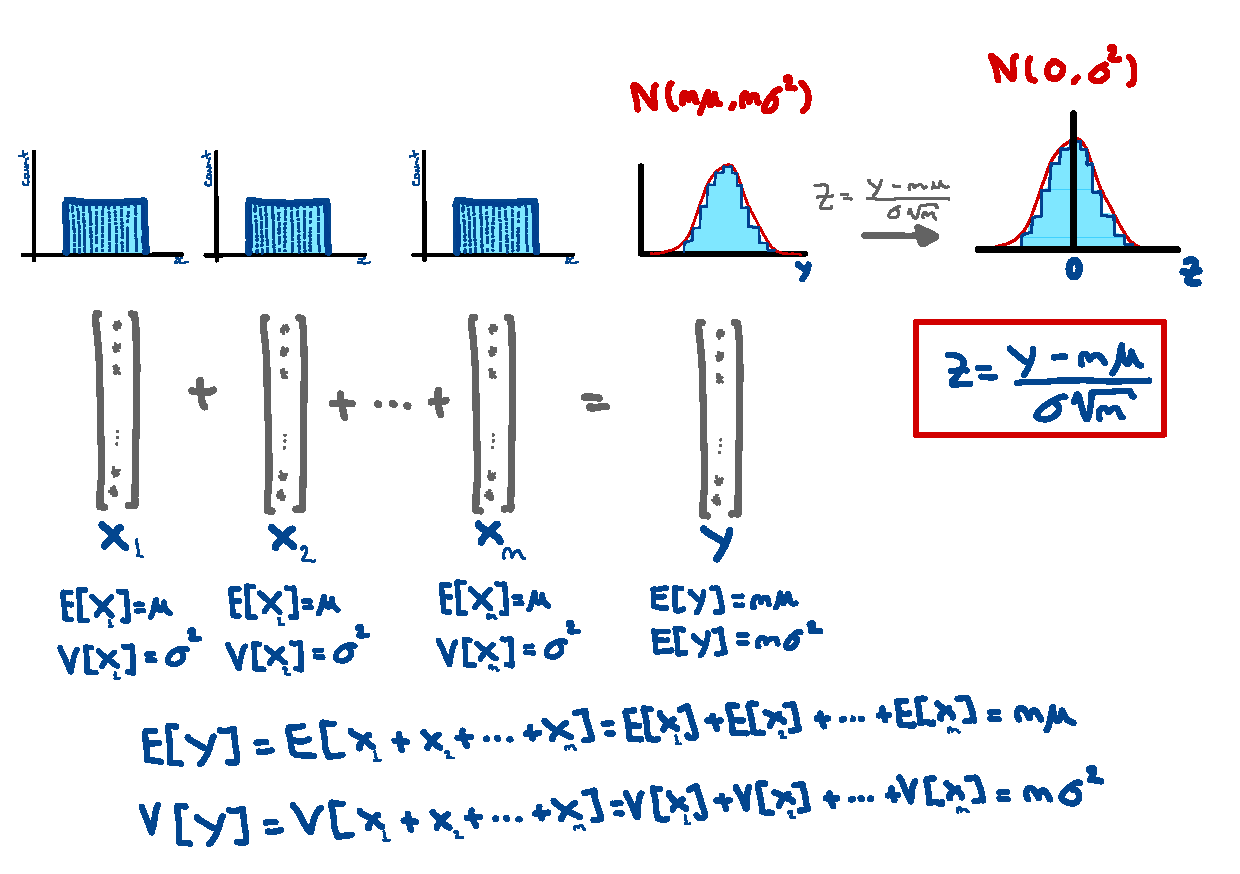
\includegraphics[width=1\textwidth]{slides/figures/clt_examples.pdf}
    \end{figure}
\end{frame}



\begin{frame}
    \frametitle{Hypothesis Testing}

    A statistical hypothesis is a statement either about the parameters of a 
    probability distribution or the parameters of a model.



    \begin{itemize}

        \item Given two experiments with mean $\mu_1$ and $\mu_2$. We can reflects some conjecture
        about the problem situation.
        $$H_0: \mu_1 = \mu_2$$
        $$H_1: \mu_1\neq\mu_2$$

        \item The statement $H_0: \mu_1=\mu_2$ is called the \textbf{null hypothesis} and
        should be always \textbf{equal}.
        \item otherwise, $H_1: \mu_1\new\mu_2$ is called the \textbf{alternative hypothesis}.
    \end{itemize}
\end{frame}



\begin{frame}
    \frametitle{Hypothesis Testing}

    To test a hypothesis, we devise a procedure for

    \begin{itemize}
        \item Taking a random sample,
        \item computing an appropriate \textbf{test statistic},
        \item and then \textbf{rejecting or failing to reject} the null hypothesis $H_0$ based on 
        the computed value of the test statistic. 


    \end{itemize}

    Rejecting the \textbf{null hypothesis}:
    \begin{itemize}
        \item The set of values for the test statistic that leads to \textbf{rejection of $H_0$} 
        is called the \textbf{critical region} or rejection region for the test.
        \item Two kinds of errors may be committed when testing hypotheses.
    \end{itemize}
    
\end{frame}


\begin{frame}
    \frametitle{Hypothesis Testing: Error Types}
    \begin{itemize}
        \item If the null hypothesis is rejected when it is true, a 
        type I error has occurred. 
        $$\alpha = P(\text{type I error}) = P(\text{reject $H_0$}|\text{$H_0$ is true})$$

        where $\alpha$ is called the \textbf{significance level} of the test,

        \item If the null hypothesis is not rejected when it is false, a type II 
        error has been made.

        $$\beta = P(\text{type II error}) = P(\text{accept $H_0$}|\text{$H_0$ is false})$$

        \item Sometimes it is more convenient to work with the \textbf{power} of the test, where

        $$\text{Power} = 1 - \beta = P(\text{reject $H_0$}|\text{$H_0$ 0s false})$$
    \end{itemize}
\end{frame}

\begin{frame}
    \frametitle{Hypothesis Testing: Error Types}
    \begin{figure}
        \centering
        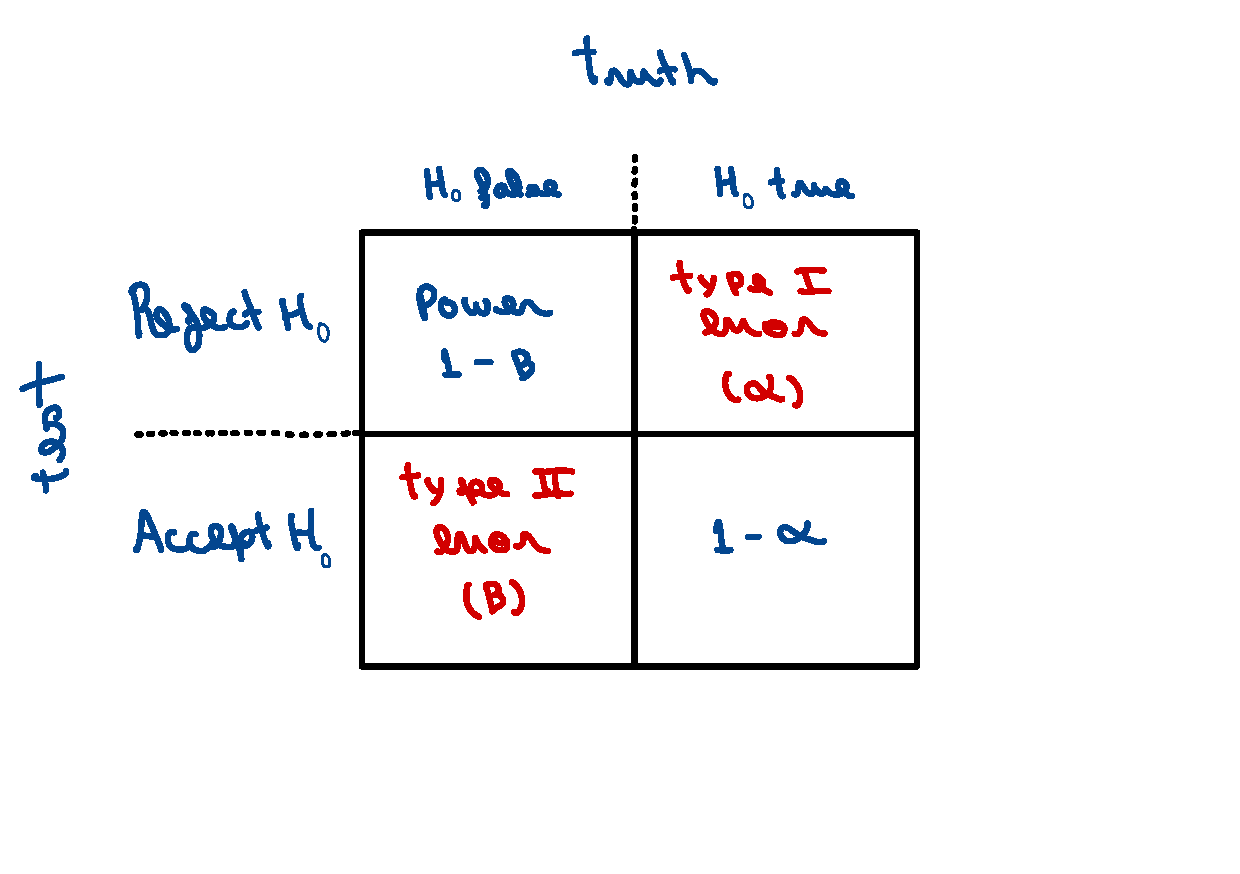
\includegraphics[width=1\textwidth]{slides/figures/error_table.pdf}
    \end{figure}
\end{frame}

\begin{frame}
    \frametitle{Hypothesis Testing: P-Value}
    
 

    \begin{definition}

    \begin{itemize}
        \item A p-value is a statistical measurement used to validate a hypothesis against observed data.

        \item In a significance test, the null hypothesis $H_{0}$ is rejected if the p-value 
        is less than or equal to a predefined threshold value $\alpha$, which is referred to 
        as the significance level.
    \end{itemize}
    
    \end{definition}
    
    Intuitively, if the P-Value is small, it means that the observed data is very unlikely to have occurred under $H_0$
    %Let's use one of the most famous statistical test ($\chi^2$ goodness of fit) to elucitate the 
    %p-value.
\end{frame}



\begin{frame}
    \frametitle{Hypothesis Testing: Chi-Square Goodness of Fit Test}

    \begin{itemize}
        \item The Chi-square goodness of fit test is a statistical hypothesis test used to determine 
        whether a variable is likely to come from a specified distribution or not.

        $$\chi^{2}_{df} = \sum_{i=1}^{n}\frac{(x_i - E[x_i])^2}{E[x_i]}$$

        where $df$ is the degrees of freedom and $n$ is the number of observations.

        \item Data values that are a simple random sample from the full population.

        \item Categorical or nominal data. The Chi-square goodness of fit test is not appropriate for 
        continuous data. Use histograms instead where each bin (range value) is a categorial class.

        \item A data set that is large enough so that at least 30 values are expected in 
        each of the observed data categories. 

    \end{itemize}
\end{frame}


\begin{frame}
    \frametitle{Chi-Square Goodness of Fit Test: Birth Example}
    \begin{figure}
        \centering
        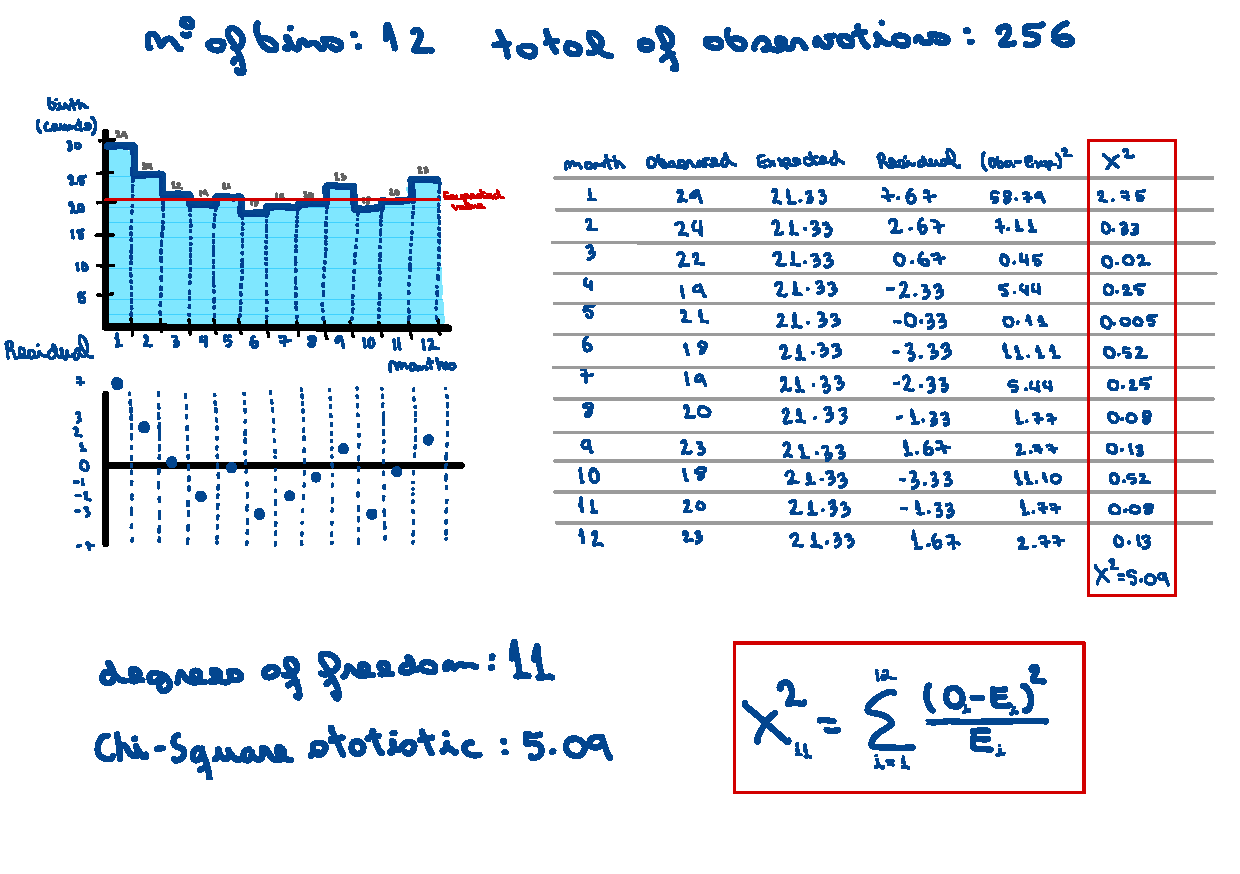
\includegraphics[width=0.9\textwidth]{slides/figures/chi2_example_one.pdf}
    \end{figure}
    Degrees of freedom for Chi-square goodness of fit test is equal to the number of groups (bins) minus one.

\end{frame}

\begin{frame}
    \frametitle{Chi-Square Goodness of Fit Test: Birth Example}


    \begin{itemize}
        \item Now, let's test the hypothesis with 5\% of significance level (or 95\% of confidence)

        $$H_0: \text{The births are uniformly distributed}$$
        $$H_1: \text{The births are not uniformly distributed.}$$

        \item To reject the null hypothesis we need to find the p-value for the chi-square test.

        \item Using the chi-square calculator with significance level ($\alpha$) of 0.05 we have:
        $$\chi^{2}_{11} = 5.09~{\color{red}\Rightarrow~\text{p-value} = 0.92673}$$

        \item Since the p-value is higher than $\alpha$, we can \textbf{accept the null hypothesis}



    \end{itemize}
   


\end{frame}






\begin{frame}
    \frametitle{Bayesian Statistical Inference}


    \begin{itemize}
        \item The goal is to draw inferences about the \textbf{unknown} variable $X$
        by observing a related random variable $Y$. The unknown variable is modeled as a random
        variable $X$, with \textbf{prior distribution}

        $$f_X(x)\text{, if $X$ is continuous,}$$
        $$P_X(x)\text{, if $X$ us discrete}$$

        \item After observing the value of the random variable $Y$, we find the
        \textbf{posterior} distribution of $X$. This is the conditional pdf (or pmf) of $X$ giben $Y=y$

        $$f_{X|Y}(x|y)~~\text{or}~~P_{X|Y}(x|y)$$

        \item The posterior distribution is usually fount using \textbf{Bayes' formula}. Using the posterior
        distribution, we can then find the point or interval estimates of $X$.

    \end{itemize}

\end{frame}


\begin{frame}
    \frametitle{Bayesian Statistical Inference}


    \begin{itemize}
        \item Let $X$ be the random variable whose value \textbf{we try to estimate}. Let $Y$ be the \textbf{observed random variable}. 

        \item That is, we have observed $Y=y$, and we would like to estimate $X$. Assuming both $X$ and $Y$ are discrete, we can write
        \small
        $$P(X=x|Y=y) = \frac{P(X=x, Y=y)}{P(Y=y)} = \frac{P(Y=y|X=x)P(X=x)}{P(Y=y)}$$
        
        The above equation, as we have seen before, is just one way of writing Bayes' rule

        \item For the continuous case we can write:

        $$f_{\theta|Y}(x|y) = \frac{f_{X|\theta}(x|\theta)f_{\theta}(\theta)}{f_X(x)}$$
    \end{itemize}

\end{frame}



\end{document}